%iffalse
\let\negmedspace\undefined
\let\negthickspace\undefined
\documentclass[journal,12pt,onecolumn]{IEEEtran}
\usepackage{cite}
\usepackage{amsmath,amssymb,amsfonts,amsthm}
\usepackage{algorithmic}
\usepackage{graphicx}
\usepackage{textcomp}
\usepackage{xcolor}
\usepackage{txfonts}
\usepackage{listings}
\usepackage{enumitem}
\usepackage{mathtools}
\usepackage{gensymb}
\usepackage{comment}
\usepackage[breaklinks=true]{hyperref}
\usepackage{tkz-euclide} 
\usepackage{listings}
\usepackage{gvv}                                        
%\def\inputGnumericTable{}                                 
\usepackage[latin1]{inputenc}     
\usepackage{xparse}
\usepackage{color}                                            
\usepackage{array}                                            
\usepackage{longtable}                                       
\usepackage{calc}                                             
\usepackage{multirow}
\usepackage{multicol}
\usepackage{hhline}                                           
\usepackage{ifthen}                                           
\usepackage{lscape}
\usepackage{tabularx}
\usepackage{array}
\usepackage{float}
\newtheorem{theorem}{Theorem}[section]
\newtheorem{problem}{Problem}
\newtheorem{proposition}{Proposition}[section]
\newtheorem{lemma}{Lemma}[section]
\newtheorem{corollary}[theorem]{Corollary}
\newtheorem{example}{Example}[section]
\newtheorem{definition}[problem]{Definition}
\newcommand{\BEQA}{\begin{eqnarray}}
\newcommand{\EEQA}{\end{eqnarray}}
\newcommand{\define}{\stackrel{\triangle}{=}}
\theoremstyle{remark}
\newtheorem{rem}{Remark}
% Marks the beginning of the document
\begin{document}
\title{Assignment 1}
\author{EE25Btech11058 - Tangellapalli Mohana Krishna Sushma}
\maketitle
\renewcommand{\thefigure}{\theenumi}
\renewcommand{\thetable}{\theenumi}
\begin{enumerate}

    \item Which of the following is \textbf{NOT} a property of an $n \times n$ singular matrix?  
    \hfill{\brak{\text{MT 2010}}}
    \begin{enumerate}[label=(\Alph*)]
        \item Rank = n
        \item Linearly dependent row vectors
        \item Zero diagonal in Gauss elimination
        \item Linearly dependent column vectors
    \end{enumerate}

    \item Which of the following is an iterative technique to solve a linear system of equations? 
    \hfill{\brak{\text{MT 2010}}}
    \begin{enumerate}[label=(\Alph*)]
    \begin{multicols}{2}
        \item Gaussian elimination
        \item LU decomposition
        \item Newton-Raphson
        \item Jacobi method
    \end{multicols}    
    \end{enumerate}

    \item Given the data set \{27.90, 34.70, 64.40, 18.92, 47.60, 39.68\}, the median value for the data set is 
    \hfill{\brak{\text{MT 2010}}}
    \begin{enumerate}[label=(\Alph*)]
    \begin{multicols}{4}
        \item $36.9$
        \item $37.19$
        \item $38.86$
        \item $54.4$
    \end{multicols}
    \end{enumerate}

    \item Which of the following is typical form of a wave equation? 
    \hfill{\brak{\text{MT 2010}}}
    \begin{enumerate}[label=(\Alph*)]
    \begin{multicols}{2}
        \item $x^2 \frac{d^2 u}{dx^2} + x \frac{du}{dx} + u = 0$
        \item $\nabla^2 u = 0$
        \item $\nabla^2 u = \frac{a^2}{\partial t^2} \frac{\partial^2 u}{\partial t^2}; \quad a>0$
        \item $\nabla^2 u = a \frac{\partial u}{\partial t}; \quad a>0$
    \end{multicols}
    \end{enumerate}

    \item A vector makes angles $\alpha, \beta$ and $\gamma$ with the three axes $x, y$ and $z$, respectively.  
    The value of $\cos^2 \alpha + \cos^2 \beta + \cos^2 \gamma$ is  
    \hfill{\brak{\text{MT 2010}}}
    \begin{enumerate}[label=(\Alph*)]
    \begin{multicols}{4}
        \item $-1$
        \item $0$
        \item $1$
        \item not determinable
    \end{multicols}
    \end{enumerate}

    \item Which of the following is \textbf{NOT} a solid state welding process?  
    \hfill{\brak{\text{MT 2010}}}
    \begin{enumerate}[label=(\Alph*)]
    \begin{multicols}{2}
        \item Friction stir welding
        \item Explosive welding
        \item Ultrasonic welding
        \item Flux cored arc welding
    \end{multicols}
    \end{enumerate}

    \item In a homogeneous system (with $c$ as the number of components) in equilibrium the total number of independent intensive thermodynamic variables is  
    \hfill{\brak{\text{MT 2010}}}
    \begin{enumerate}[label=(\Alph*)]
    \begin{multicols}{4}
        \item $c-1$
        \item $c$
        \item $c+1$
        \item $c+2$
    \end{multicols}
    \end{enumerate}

    \item Which of these metals \textbf{CANNOT} be electroplated from aqueous electrolyte?  
    \hfill{\brak{\text{MT 2010}}}
    \begin{enumerate}[label=(\Alph*)]
    \begin{multicols}{4}
        \item Al
        \item Cu
        \item Ni
        \item Zn
    \end{multicols} 
    \end{enumerate}

    \item At steady state and when the inner and outer walls of a long hollow cylinder are kept at two different temperatures, the unidirectional temperature variation along the thickness of the wall is  
    \hfill{\brak{\text{MT 2010}}}
    \begin{enumerate}[label=(\Alph*)]
    \begin{multicols}{4}
        \item linear
        \item parabolic
        \item logarithmic
        \item constant
    \end{multicols}  
    \end{enumerate}
    

    \item In a basic oxygen furnace, under appropriate conditions, which of the following statements is NOT correct?
    \hfill{\brak{\text{MT 2010}}}
    \begin{enumerate}[label=(\Alph*)]
        \item Carbon can be removed in preference to P and S
        \item Phosphorus can be removed in preference to C and S
        \item Sulphur can be removed in preference to C and P
        \item Carbon and phosphorus can be removed in preference to S
    \end{enumerate}
    \item The miller indices of the direction common to the planes(11)and(110) in a cubic system is 
    \hfill{\brak{\text{MT 2010}}}
    \begin{enumerate}[label=(\Alph*)]
     \begin{multicols}{4} 
    \item [A.] [111]
    \item [B.] [110]
    \item [C.] [1$\overline{1}$0]
    \item [D.] [1$\overline{1}$1]
    \end{multicols}
    \end{enumerate} 

    

    \item In continuous casting of steel, the mould is subjected to vertical oscillations in order to
    \hfill{\brak{\text{MT 2010}}}
    \begin{enumerate}[label=(\Alph*)]
        \item allow easy flotation of inclusions
        \item ensure good casting homogeneity
        \item increase the heat transfer rate from the steel to the mould
        \item prevent the skin sticking to the mould
    \end{enumerate}
    


    \item The engineering stress-strain curve for a ceramic material is
    \hfill{\brak{\text{MT 2010}}}
    \begin{enumerate}[label=(\Alph*)]
    \begin{multicols}{4}
        \item parabolic
        \item exponential
        \item logarithmic
        \item linear
    \end{multicols} 
    \end{enumerate}
    
    \item Which of the following statements regarding Kroll's process is NOT correct?
    \hfill{\brak{\text{MT 2010}}}
    \begin{enumerate}[label=(\Alph*)]
        \item Pure metal chlorides serve as main raw material
        \item Reduction is done by sodium
        \item Reduction chamber should be free of oxygen
        \item It is used for extraction of titanium and zirconium
    \end{enumerate}

    \item The energy dispersive spectrometer (EDS) in an electron microscope does chemical analysis by analysing the energy of
    \hfill{\brak{\text{MT 2010}}}
    \begin{enumerate}[label=(\Alph*)]
    \begin{multicols}{2}
        \item secondary electrons
        \item auger electrons
        \item charecteristics X-rays
        \item back-scattered electrons
    \end{multicols}    
    \end{enumerate}

    \item In heterogeneous nucleation, the radius of the critical nucleus does NOT depend on
    \hfill{\brak{\text{MT 2010}}}
    \begin{enumerate}[label=(\Alph*)]
        \item contact angle
        \item undercooling
        \item the surface energy of the interface between the product and parent phases
        \item enthalpy change per unit volume of the product phase
    \end{enumerate}

    \item The third peak in the X-ray diffraction pattern of a polycrystalline BCC metal is
    \hfill{\brak{\text{MT 2010}}}
    \begin{enumerate}[label=(\Alph*)]
    \begin{multicols}{4}
        \item (111)
        \item (110)
        \item (211)
        \item (220)
    \end{multicols} 
    \end{enumerate}

    \item Number of slip systems in an ideal close packed hexagonal structure is
    \hfill{\brak{\text{MT 2010}}}
    \begin{enumerate}[label=(\Alph*)]
    \begin{multicols}{4}
        \item $3$
        \item $12$
        \item $24$
        \item $48$
    \end{multicols}
    \end{enumerate}
    \item square of $9~\text{mm}^2$ area is subjected to simple shear displacement $\sqrt{3}$~mm along x-direction, as shown below
    \begin{figure}[H]
    \centering
    \includegraphics[width=0.25\columnwidth]{figs/19.png}
            
\label{fig:19.png}
        \end{figure}
    The shear strain imparted will be
    \hfill{\brak{\text{MT 2010}}} 
    \begin{enumerate}[label=(\Alph*)]
    \begin{multicols}{4}
    \item[(A)] $1/3$
    \item[(B)] $\frac{1}{\sqrt{3}}$
    \item[(C)] $\sqrt{3}$
    \item[(D)] $3$
    \end{multicols}
    \end{enumerate}
    \item During metal casting of a slab, the thickness of solid formed after time $t$ is proportional to
    \hfill{\brak{\text{MT 2010}}}
    \begin{enumerate}[label=(\Alph*)]
    \begin{multicols}{4}
    \item $t^{3}$
    \item $t^{1/2}$
    \item $t$
    \item $t^{2}$
    \end{multicols}
    \end{enumerate}

    \item Which of the following is a suitable method to remove hydrogen from molten aluminium?
    \hfill{\brak{\text{MT 2010}}}
    \begin{enumerate}[label=(\Alph*)]
    \item Expose flowing melt to vacuum
    \item Bubble humidified argon gas through the melt
    \item Increase melt temperature
    \item Cover melt surface with a flux
    \end{enumerate}

    \item Driving force for grain growth after completion of recrystallization is
    \hfill{\brak{\text{MT 2010}}}
    \begin{enumerate}[label=(\Alph*)]
    \begin{multicols}{2}
    \item stored energy of cold work
    \item dislocation density in the crystal
    \item vacancy concentration
    \item grain boundary curvature
    \end{multicols}
    \end{enumerate}

    \item Which of the following partial derivative is equal to $\left(\frac{\partial S}{\partial P}\right)_T$?
    \hfill{\brak{\text{MT 2010}}}
    \begin{enumerate}[label=(\Alph*)]
    \begin{multicols}{4}
    \item $-\left(\frac{\partial V}{\partial T}\right)_P$
    \item $\left(\frac{\partial S}{\partial V}\right)_T$
    \item $\left(\frac{\partial V}{\partial T}\right)_S$
    \item $-\left(\frac{\partial S}{\partial V}\right)_T$
    \end{multicols}
    \end{enumerate}

    \item Which of the following are NOT commercially manufactured by powder metallurgy?
    \hfill{\brak{\text{MT 2010}}}
    \begin{enumerate}[label=(\Alph*)]
    \begin{multicols}{2}
    \item aircraft brake pads
    \item tungsten carbide based cutting tools
    \item self lubricating bearings
    \item turbine blades
    \end{multicols}
    \end{enumerate}

    \item Two fluids of densities $\rho_1$ and $\rho_2$ are flowing at velocities $v_1$ and $v_2$, respectively, through smooth pipes of identical diameter and pressure per unit length. When the friction factor is same, the ratio $\rho_1/\rho_2$ is equal to
    \hfill{\brak{\text{MT 2010}}}
    \begin{enumerate}[label=(\Alph*)]
    \begin{multicols}{4}
    \item $v_1/v_2$
    \item $(v_1/v_2)^2$
    \item $(v_2/v_1)^2$
    \item $(v_2/v_1)^{1/2}$
    \end{multicols}
    \end{enumerate}
    

    

    \item Determine the radius (in m) of a cylinder of volume $200~\mathrm{m}^3$ that has the least surface area
    \hfill{\brak{\text{MT 2010}}}
    \begin{enumerate}[label=(\Alph*)]
    \begin{multicols}{4}
    \item $2.302$
    \item $3.142$
    \item $3.169$
    \item $7.233$
    \end{multicols}
    \end{enumerate}

    \item Given the polynomial $x^3 - 3x^2 + 4x - 2.5 = 0$\\
    Starting from a guess value $x = 0$, what will be the value of $x$ after iterating twice using the Newton-Raphson method.
    \hfill{\brak{\text{MT 2010}}}
    \begin{enumerate}[label=(\Alph*)]
    \begin{multicols}{4}
    \item $0.625$
    \item $1.278$
    \item $1.441$
    \item $1.562$
    \end{multicols}
    \end{enumerate}

    \item The probability of obtaining ``head'' $n$ times, on tossing an unbiased coin $N$ times, is given by
    \hfill{\brak{\text{MT 2010}}}
    \begin{enumerate}[label=(\Alph*)]
    \begin{multicols}{4}
    \item ${}^N C_n \left(\frac{1}{2}\right)^N$
    \item $\frac{n}{N}$
    \item $\left(\frac{1}{2}\right)^N$
    \item ${}^N P_n \left(\frac{1}{2}\right)^N$
    \end{multicols}
    \end{enumerate}

    \item $\displaystyle \lim_{x \to 0} \frac{\sin^2 a x}{\sin^2 x}$ is
    \hfill{\brak{\text{MT 2010}}}
    \begin{enumerate}[label=(\Alph*)]
    \begin{multicols}{4}
    \item $a^2$
    \item $0$
    \item $1$
    \item undefined
    \end{multicols}
    \end{enumerate}
    



    \item Solution of the equation $2x \dfrac{dy}{dx} + 3y = 0$ is
    \hfill{\brak{\text{MT 2010}}}
    \begin{enumerate}[label=(\Alph*)]
    \begin{multicols}{4}
    \item $x\,y^{2}$
    \item $x^{3}y^{2}$
    \item $x\,y^{2}$
    \item $x^{3}y^{2}$
    \end{multicols}
    \end{enumerate}

    \item Match the metallurgical processes in \textbf{Group I} with their corresponding reactor types in \textbf{Group II}.
    
    \begin{minipage}{0.45\textwidth}
    \textbf{Group I}
    \begin{enumerate}
    \item P. Roasting of sulphide concentrate
    \item Q. LD steel making
    \item R. Dwight-Lloyd sintering
    \item S. Zinc extraction
    \end{enumerate}
    \end{minipage}%
    \begin{minipage}{0.45\textwidth}
    \textbf{Group II}
    \begin{enumerate}
    \item 1. Pneumatic reactor
    \item 2. Retort
    \item 3. Travelling grate reactor
    \item 4. Fluidized bed reactor
    \end{enumerate}
    \end{minipage}
    \hfill{\brak{\text{MT 2010}}}
    \begin{enumerate}[label=(\Alph*)]
    \begin{multicols}{2}
    \item P-3, Q-2, R-4, S-1
    \item P-4, Q-1, R-3, S-2
    \item P-3, Q-4, R-2, S-1
    \item P-4, Q-1, R-2, S-3
    \end{multicols}
    \end{enumerate}


    \item The theoretical density of an FCC metal with atomic radius and atomic weight of 0.144~nm and 197~g~mol$^{-1}$, respectively, is approximately (in kg m$^{-3}$)
    \hfill{\brak{\text{MT 2010}}}
    \begin{enumerate}[label=(\Alph*)]
    \begin{multicols}{4}
    \item $18110$
    \item $18300$
    \item $19360$
    \item $19890$
    \end{multicols}
    \end{enumerate}

    \item In a binary system, the difference in chemical potentials of two components ($\mu_A-\mu_B$) is equal to
    \hfill{\brak{\text{MT 2010}}}
    \begin{enumerate}[label=(\Alph*)]
    \begin{multicols}{4}
    \item $\frac{d G_A}{d x}$
    \item $0$
    \item $(1-x)\frac{d G_A}{d x}$
    \item $-\frac{d G_B}{d x}$
    \end{multicols}
    \end{enumerate}

    \item The temperature of a gas flowing in a long duct as measured by a thermocouple (having an emissivity of 0.5) is 800~K. The internal wall surface of the duct is at a temperature of 500~K. The convective heat transfer coefficient between the gas and the tip of the thermocouple is 100~W\,m$^{-2}$K$^{-1}$. The actual gas temperature is approximately
    \hfill{\brak{\text{MT 2010}}}
    \begin{enumerate}[label=(\Alph*)]
    \begin{multicols}{4}
    \item $400$ K
    \item $500$ K
    \item $820$ K
    \item $900$ K
    \end{multicols}
    \end{enumerate}

    \item A recrystallization process is 20\% complete after 45 s and 85\% complete after 75 s. Assuming Avrami kinetics, the value of Avrami exponent ``$n$" is
    \hfill{\brak{\text{MT 2010}}}
    \begin{enumerate}[label=(\Alph*)]
    \begin{multicols}{4}
    \item $4.19$
    \item $3.12$
    \item $2.42$
    \item $1.34$
    \end{multicols}
    \end{enumerate}
    
    \item Match the defects given in \textbf{Group I} with the suitable non-destructive evaluation technique from \textbf{Group II}.
    
    \begin{minipage}{0.45\textwidth}
    \textbf{Group I}
    \vspace{-4pt}
    \begin{enumerate}[label=(\Alph*)]
    \item P. Cracks in a flat aluminium slab
    \item Q. Subsurface porosity in a bronze casting
    \item R. Surface cracks in a steel tool
    \item S. Internal porosity in a ceramic block
    \end{enumerate}
    \end{minipage}%
    \begin{minipage}{0.45\textwidth}
    \textbf{Group II}
    \vspace{-4pt}
    
    \begin{enumerate}
    \item 1. Radiography
    \item 2. Eddy current technique
    \item 3. Ultrasonic technique
    \item 4. Magnetic particle technique
    \end{enumerate}
    \end{minipage}
    \hfill{\brak{\text{MT 2010}}}
    \begin{enumerate}[label=(\Alph*)]
    \begin{multicols}{2}
    \item P-3, Q-4, R-1, S-2
    \item P-1, Q-2, R-4, S-3
    \item P-4, Q-1, R-3, S-1
    \item P-1, Q-3, R-4, S-2
    \end{multicols}
    \end{enumerate}
    \item Silicon is doped with arsenic (concentration $10^{20}$ atoms m$^{-3}$). At room temperature, the electron and hole mobilities in Si are 0.14 m$^2$V$^{-1}$s$^{-1}$ and 0.05 m$^2$V$^{-1}$s$^{-1}$, respectively. The conductivity, (Ωm)$^{-1}$, at room temperature for Si doped with As is
    \hfill{\brak{\text{MT 2010}}}
    \begin{enumerate}[label=(\Alph*)]
    \begin{multicols}{4}
    \item $0.11$
    \item $0.96$
    \item $2.24$
    \item $2.72$
    \end{multicols}
    \end{enumerate}
    \item Four eutectoid steel samples W, X, Y and Z are austenized and then subjected to normalizing, quenching, martempering and austempering treatments, respectively. Which of the following statements is \textbf{NOT} correct?
    \hfill{\brak{\text{MT 2010}}}
    \begin{enumerate}[label=(\Alph*)]
    \item The microstructure of sample W will be fully pearlitic
    \item The microstructure of sample X will be untempered martensite
    \item The microstructure of sample Y will be tempered martensite
    \item The microstructure of sample Z will be bainitic
    \end{enumerate}

    \item The difference in reversible potential between oxygen reduction reaction and hydrogen evolution reaction at any pH in an aqueous electrolyte is\\
    \textit{(given standard reduction potentials for hydrogen evolution reaction: $ E^0_{H_2/H^+} = 0$ V. SHE and oxygen reduction reaction: $E^0_{O_2/H_2O}=0.4$ V. SHE. Also, $p_{H_2} = p_{O_2} = 1$ atm)}
    \hfill{\brak{\text{MT 2010}}}
    \begin{enumerate}[label=(\Alph*)]
    \begin{multicols}{4}
    \item $0$ V
    \item $0.41$ V
    \item $0.82$ V
    \item $1.23$ V
    \end{multicols}
    \end{enumerate}

    \item \textbf{Assertion a:} Hardenability of steel can be increased by adding certain alloying elements.
    \textbf{Reason r:} The alloying elements can provide a fine dispersion of alloy carbides.
    \hfill{\brak{\text{MT 2010}}}
    \begin{enumerate}[label=(\Alph*)]
    \item Both a and r are true but r is not a correct reason for a
    \item Both a and r are false
    \item a is true but r is false
    \item Both a and r are true and r is a correct reason for a
    \end{enumerate}

    \item Consider the following collection of polymer chains:

    \begin{tabular}{ll}
    Number of molecules: & 10 \hspace{3mm} 5 \hspace{3mm} 4 \hspace{3mm} 2 \hspace{3mm} 1 \\
    Molecular weight (g mol$^{-1}$): & 2800 \hspace{2mm} 3000 \hspace{2mm} 1200 \hspace{2mm} 3600 \hspace{2mm} 1000
    \end{tabular}

    Met unit is ethylene. Atomic weights: carbon (12) and hydrogen (1). Calculate number average degree of polymerization.
    \hfill{\brak{\text{MT 2010}}}
    \begin{enumerate}[label=(\Alph*)]
    \begin{multicols}{4}
    \item $32.32$
    \item $90.91$
    \item $106.61$
    \item $116.13$
    \end{multicols}
    \end{enumerate}

    \item At 910$^\circ$C, $\gamma$-Fe transforms to $\alpha$-Fe resulting in a percentage volume expansion of
    \hfill{\brak{\text{MT 2010}}}
    \begin{enumerate}[label=(\Alph*)]
    \begin{multicols}{4}
    \item $5.6$
    \item $7.1$
    \item $7.6$
    \item $8.8$
    \end{multicols}
    \end{enumerate}

    \item \textbf{Group I} is a list of technologies for alternate methods of producing iron. \textbf{Group II} is a list of terms you come across in the context of these technologies. Match the items.

    \begin{minipage}{0.45\textwidth}
    \textbf{Group I}
    \vspace{-6pt}
    \begin{enumerate}
    \item[P.] MIDREX
    \item[Q.] COREX
    \item[R.] SL/RN
    \item[S.] HyL-I
    \end{enumerate}
    \end{minipage}%
    \hfill
    \begin{minipage}{0.45\textwidth}
    \textbf{Group II}
    \vspace{-6pt}
    \begin{enumerate}
    \item[1.] Retort
    \item[2.] Rotary kiln
    \item[3.] Smelting reduction
    \item[4.] Shaft furnace
    \end{enumerate}
    \end{minipage}
    \hfill{\brak{\text{MT 2010}}}
    \begin{enumerate}[label=(\Alph*)]
    \begin{multicols}{2}
    \item P-3, Q-1, R-2, S-4
    \item P-1, Q-3, R-2, S-4
    \item P-4, Q-2, R-1, S-3
    \item P-4, Q-3, R-2, S-1
    \end{multicols}
    \end{enumerate}

     \item If the true stress-true strain curve of a ductile material is represented by the equation $\sigma = 1100\,\epsilon^{0.3}$, the ultimate tensile strength (engineering) will be
    \hfill{\brak{\text{MT 2010}}}
    \begin{enumerate}[label=(\Alph*)]
    \begin{multicols}{4}
    \item $853$ MPa
    \item $753$ MPa
    \item $653$ MPa
    \item $553$ MPa
    \end{multicols}
    \end{enumerate} 
    \item The maximum possible reduction in a single pass for cold rolling of a 200~mm slab is (given the coefficient of friction is 0.1 and roll diameter is 400~mm)
    \hfill{\brak{\text{MT 2010}}}
    \begin{enumerate}[label=(\Alph*)]
    \begin{multicols}{4}
    \item $5$~mm
    \item $3$~mm
    \item $2$~mm
    \item $1$~mm
    \end{multicols}
    \end{enumerate}
    \item Match the requirement from \textbf{Group I} with the suitable casting process from \textbf{Group II}.

    \begin{minipage}{0.45\textwidth}
    \textbf{Group I}
    \begin{enumerate}[label=\textbf{\Alph*.}]
    \item Good surface finish
    \item Expendable mould
    \item Heavy casting
    \item Hollow ornamental casting
    \end{enumerate}
    \end{minipage}%
    \hfill
    \begin{minipage}{0.45\textwidth}
    \textbf{Group II}
    \begin{enumerate}[label=\textbf{\arabic*.}]
    \item Slush casting
    \item Pressure die casting
    \item Investment casting
    \item Sand casting
    \end{enumerate}
    \end{minipage}
    \hfill{\brak{\text{MT 2010}}}
    \begin{enumerate}[label=(\Alph*)]
    \begin{multicols}{2}
    \item P-2, Q-3, R-4, S-1
    \item P-4, Q-3, R-1, S-4
    \item P-4, Q-2, R-4, S-1
    \item P-2, Q-1, R-3, S-4
    \end{multicols}
    \end{enumerate}

    \item  The tensile test of a sheet material exhibits 20\% elongation in length and 10\% decrease in width. The plastic strain ratio is
    \hfill{\brak{\text{MT 2010}}}
    \begin{enumerate}[label=(\Alph*)]
    \begin{multicols}{4}
    \item $2.37$
    \item $1.37$
    \item $1.17$
    \item $0.87$
    \end{multicols}
    \end{enumerate}
    \textbf{Common Data Questions}

    \textbf{Common Data for Questions 48 and 49}

    \begin{figure}[H]
        \centering
        \includegraphics[width=0.50\columnwidth]{figs/48.png}
        \label{fig:48.png}
    \end{figure}
    In the above hypothetical phase diagram, the melting point of each pure component is 1000 K and the eutectic temperature is 800 K. The eutectic is located at the equi-atomic composition. The maximum solid solubility in $\alpha$ phase is given by mole fraction $N_B = 0.1$.

    \textbf{Q.48} The freezing range (in K) of the alloy with composition $N_B=0.1$ is
    \hfill{\brak{\text{MT 2010}}}
    \begin{enumerate}[label=(\Alph*)]
    \begin{multicols}{4}
    \item $100$
    \item $130$
    \item $160$
    \item $190$
    \end{multicols}
    \end{enumerate}

    \textbf{Q.49} On cooling an alloy of composition $N_B=0.2$, the fraction of pro-eutectic $\alpha$ phase at the eutectic temperature is
    \hfill{\brak{\text{MT 2010}}}
    \begin{enumerate}[label=(\Alph*)]
    \begin{multicols}{4}
    \item $0.75$
    \item $0.65$
    \item $0.55$
    \item $0.45$
    \end{multicols}
    \end{enumerate}

    \textbf{Common Data for Questions 50 and 51}

    An aluminium alloy rod of diameter 15 mm and length 120 mm is subjected to a tensile load of 35,000 N along its axis. The Young's modulus and Poisson's ratio for aluminium are 70 GPa and 0.33 respectively.

    \textbf{Q.50} The reduction in diameter on the application of tensile load is
    \hfill{\brak{\text{MT 2010}}}
    \begin{enumerate}[label=(\Alph*)]
    \begin{multicols}{4}
    \item $0.011$ mm
    \item $0.014$ mm
    \item $0.018$ mm
    \item $0.021$ mm
    \end{multicols}
    \end{enumerate}

    \textbf{Q.51} The elastic strain energy is approximately
    \hfill{\brak{\text{MT 2010}}}
    \begin{enumerate}[label=(\Alph*)]
    \begin{multicols}{4}
    \item $200$ kJ~m$^{-3}$
    \item $240$ kJ~m$^{-1}$
    \item $280$ kJ~m$^{-3}$
    \item $320$ kJ~m$^{-3}$
    \end{multicols}
    \end{enumerate}
    

    \textbf{Linked Answer Questions}

    \bigskip

    \textbf{Statement for Linked Answer Questions 52 and 53}

    At 1200$^\circ$C the standard Gibbs energy of thermal decomposition of one mole of wustite into Fe and O$_2$ is 168 kJ.

    \noindent\textbf{Q.52} The corresponding dissociation pressure (in atm) is
    \hfill{\brak{\text{MT 2010}}}
    \begin{enumerate}[label=(\Alph*)]
    \begin{multicols}{4}
    \item[(A)] $2.51 \times 10^{-13}$
    \item[(B)] $1.22 \times 10^{-12}$
    \item[(C)] $5.09 \times 10^{-8}$
    \item[(D)] $1.13 \times 10^{-6}$
    \end{multicols}
    \end{enumerate}

    \noindent\textbf{Q.53} Given for the reaction $2$CO~$+$~O$_2 \leftrightarrow 2$CO$_2$, the standard Gibbs energy is $-310$\,kJ, what is the equivalent $\left(\dfrac{P_{\mathrm{CO}_2}}{P_{\mathrm{CO}}}\right)$
    \hfill{\brak{\text{MT 2010}}}
    \begin{enumerate}[label=(\Alph*)]
    \begin{multicols}{4}
    \item[(A)] $0.03$
    \item[(B)] $1.01$
    \item[(C)] $1.85$
    \item[(D)] $2.89$
    \end{multicols}
    \end{enumerate}

    \bigskip

    \textbf{Statement for Linked Answer Questions 54 and 55}
    \begin{center}
    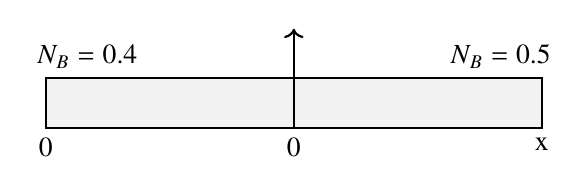
\begin{tikzpicture}[thick,scale=1.05]
    % Bar
    \draw[fill=gray!10] (-3,0) rectangle (3,0.6);
    % Compositions
    \node[above] at (-2.5,0.6) {$N_B = 0.4$};
    \node[above] at (2.5,0.6) {$N_B = 0.5$};
    % Centerline x=0
    \draw[->] (0,0) -- (0,1.2);
    % Center "0"
    \node[below] at (0,0) {0};
    % Far left "0"
    \node[below] at (-3,0) {0};
    % Far right "x"
    \node[below] at (3,0) {x};
    \end{tikzpicture}
    \end{center}

    The diffusion couple shown above is made from two A-B alloys. The initial compositions of the two alloys are indicated in the diagram. The centerline is at $x=0$. The couple is held at an elevated temperature for 40 hours. Diffusivity $D=3\times 10^{-11}$ m$^2$s$^{-1}$. Assume the diffusion couple to be infinitely long.

    \vspace{1em}
    \noindent\textbf{Q.54} Which of the parameters give the composition profile in the following form?
    \[
    C(x,t) = C_1 + C_2\,\mathrm{erf} \left( \frac{x}{2\sqrt{Dt}} \right)
    \]
    \hfill{\brak{\text{MT 2010}}}
    \begin{enumerate}[label=(\Alph*)]
    \begin{multicols}{4}
    \item[(A)] $C_1 = 0.45$, $C_2 = 0.05$
    \item[(B)] $C_1 = 0.5$, $C_2 = 0.4$
    \item[(C)] $C_1 = 0.05$, $C_2 = 0.45$
    \item[(D)] $C_1 = 0.1$, $C_2 = 0.9$
    \end{multicols}
    \end{enumerate}

    \vspace{1em}
    \noindent\textbf{Q.55} The composition at a distance $x = 2$ mm is approximately (assuming $\mathrm{erf}(x) \approx x$ for small $x$)
    \hfill{\brak{\text{MT 2010}}}
    \begin{enumerate}[label=(\Alph*)]
    \begin{multicols}{4}
    \item[(A)] $0.3$
    \item[(B)] $0.474$
    \item[(C)] $0.524$
    \item[(D)] $0.7$
    \end{multicols}
    \end{enumerate}
   

   \noindent\textbf{General Aptitude (GA) Questions}
   \textbf{Q.56} \textit{Which of the following options is the closest in meaning to the word below:}\\
   \textbf{Circuitous}
   \hfill{\brak{\text{MT 2010}}}
   \begin{enumerate}[label=(\Alph*)]
   \begin{multicols}{4}
    \item cyclic
    \item indirect
    \item confusing
    \item crooked
    \end{multicols}
    \end{enumerate}

    \textbf{Q.57} \textit{The question below consists of a pair of related words followed by four pairs of words. Select the pair that best expresses the relation in the original pair.}\\
    Unemployed : Worker
    \hfill{\brak{\text{MT 2010}}}
    \begin{enumerate}[label=(\Alph*)]
    \begin{multicols}{4}
    \item tallow : land
    \item uaware : sleeper
    \item wit : jester
    \item renovated : house
    \end{multicols}
    \end{enumerate}

    \textbf{Q.58} \textit{Choose the most appropriate word from the options given below to complete the following sentence:}\\
    \textbf{If we manage to \underline{\hspace{2cm}} our natural resources, we would leave a better planet for our children.}
    \hfill{\brak{\text{MT 2010}}}
    \begin{enumerate}[label=(\Alph*)]
    \begin{multicols}{4}
    \item uphold
    \item restrain
    \item cherish
    \item conserve
    \end{multicols}
    \end{enumerate}

    \textbf{Q.59} \textit{Choose the most appropriate word from the options given below to complete the following sentence:}\\
    \textbf{His rather casual remarks on politics \underline{\hspace{2cm}} his lack of seriousness about the subject.}
    \hfill{\brak{\text{MT 2010}}}
    \begin{enumerate}[label=(\Alph*)]
    \begin{multicols}{4}
    \item masked
    \item belied
    \item betrayed
    \item suppressed
    \end{multicols}
    \end{enumerate}

    \textbf{Q.60} 25 persons are in a room. 15 of them play hockey, 17 of them play football and 10 of them play both hockey and football. Then the number of persons playing neither hockey nor football is:
    \hfill{\brak{\text{MT 2010}}}
    \begin{enumerate}[label=(\Alph*)]
    \begin{multicols}{4}
    \item $2$
    \item $17$
    \item $3$
    \item $13$
    \end{multicols}
    \end{enumerate}

    \medskip

    \noindent\textbf{Q.61 -- Q.65 carry two marks each.}

    \vspace{3mm}
   
    \textbf{Q.61} Modern warfare has changed from large scale clashes of armies to suppression of civilian populations. Chemical agents that do their work silently appear to be suited to such warfare; and regretfully, there exist people in military establishments who think that chemical agents are useful tools for their cause.

    \emph{Which of the following statements best sums up the meaning of the above passage:}
    \hfill{\brak{\text{MT 2010}}}
    \begin{enumerate}[label=(\Alph*)]
    \item Modern warfare has resulted in civil strife.
    \item Chemical agents are useful in modern warfare.
    \item Use of chemical agents in warfare would be undesirable.
    \item People in military establishments like to use chemical agents in war.
    \end{enumerate}
    \noindent\textbf{Q.62} If $137 + 276 = 435$ how much is $731 + 672$?
    \hfill{\brak{\text{MT 2010}}}
    \begin{enumerate}[label=(\Alph*)]
    \begin{multicols}{4}
    \item $534$
    \item $1403$
    \item $1623$
    \item $1513$
    \end{multicols}
    \end{enumerate}

    \noindent\textbf{Q.63} 5 skilled workers can build a wall in 20 days; 8 semi-skilled workers can build a wall in 25 days; 10 unskilled workers can build a wall in 30 days. If a team has 2 skilled, 6 semi-skilled and 5 unskilled workers, how long will it take to build the wall?
    \hfill{\brak{\text{MT 2010}}}
    \begin{enumerate}[label=(\Alph*)]
    \begin{multicols}{4}
    \item $20$ days
    \item $18$ days
    \item $16$ days
    \item $15$ days
    \end{multicols}
    \end{enumerate}

    \noindent\textbf{Q.64} Given digits 2, 2, 3, 3, 3, 4, 4, 4, 4 how many distinct 4 digit numbers greater than 3000 can be formed?
    \hfill{\brak{\text{MT 2010}}}
    \begin{enumerate}[label=(\Alph*)]
    \begin{multicols}{4}
    \item $50$
    \item $51$
    \item $52$
    \item $54$
    \end{multicols}
    \end{enumerate}

    \noindent\textbf{Q.65} Hari (H), Gita (G), Irfan (I) and Saira (S) are siblings (i.e. brothers and sisters). All were born on 1\textsuperscript{st} January. The age difference between any two successive siblings (that is born one after another) is less than 3 years. Given the following facts:
    \begin{itemize}
    \item[(i)]  Hari's age + Gita's age = Irfan's age + Saira's age.
    \item[(ii)] The age difference between Gita and Saira is 1 year. However, Gita is not the oldest and Saira is not the youngest.
    \item[(iii)] There are no twins.
    \end{itemize}
     In what order were they born (oldest first)?
     \hfill{\brak{\text{MT 2010}}}
     \begin{enumerate}[label=(\Alph*)]
     \begin{multicols}{4}
     \item HSIG
     \item SGHI
     \item IGSH
     \item IHSG
     \end{multicols}
     \end{enumerate}

     \vspace{1cm}
     \begin{center}
     \textbf{END OF THE QUESTION PAPER}
     \end{center}
     

    
    \end{enumerate}
    \end{document}
    